\documentclass{article}
%%\documentclass[draft]{article}

\usepackage{arxiv}

\usepackage[utf8]{inputenc} % allow utf-8 input
\usepackage[T1]{fontenc}    % use 8-bit T1 fonts
\usepackage[hidelinks]{hyperref}       % hyperlinks
\usepackage{url}            % simple URL typesetting
\usepackage{booktabs}       % professional-quality tables
\usepackage{amsfonts}       % blackboard math symbols
\usepackage{nicefrac}       % compact symbols for 1/2, etc.
\usepackage{microtype}      % microtypography
\usepackage{lipsum}

\usepackage{graphicx}
\usepackage{subfig}
\usepackage{xcolor}
\usepackage{listings}

\usepackage{tikz,pgfplots}

%% code color styling
\definecolor{codegreen}{rgb}{0,0.6,0}
\definecolor{codegray}{rgb}{0.5,0.5,0.5}
\definecolor{codepurple}{rgb}{0.58,0,0.82}
\definecolor{backcolour}{rgb}{0.95,0.95,0.92}
\lstdefinestyle{mystyle}{
    backgroundcolor=\color{backcolour},   
    commentstyle=\color{codegreen},
    keywordstyle=\color{magenta},
    numberstyle=\tiny\color{codegray},
    stringstyle=\color{codepurple},
    basicstyle=\ttfamily\footnotesize,
    breakatwhitespace=false,         
    breaklines=true,                 
    captionpos=b,                    
    keepspaces=true,                 
    %numbers=left,                    
    %numbersep=5pt,                  
    showspaces=false,                
    showstringspaces=false,
    showtabs=false,                  
    tabsize=2
}
\lstset{style=mystyle}





\title{AI Project 3: Node Insertion Heuristic}

\author{
  Robert Max Williams\\
  Department of Computer Science\\
  University of Louisville
  Louisville, KY 40208 \\
  \texttt{r0will21@louisville.edu} \\
}

\begin{document}
\maketitle

%%\begin{abstract}
%%Oh dear I really don'y need ab abstruct sahshshshsh
%%\end{abstract}




\section{Introduction}

The previous algorithms, brute force and tree search, both suffer from exponential explosion. More precisely, they run
in $N!$ and $B^{N}$ time, respectively, where $B$ is the branching factor and $N$ is the number of nodes in the solution.
In this project, we investigate greedy algorithms, which are applied to traveling salesperson problems with
$N=30$ and $N=40$, which were unfeasible for previous algorithms.

\section{Approach}
\label{sec:approach}

A Hamiltonian path of length 3 is selected from the points. The selection of the starting points is important, it can cause as
much as a 20\% difference in the length of the solution path. I used two different approaches for selecting the starting
points. The first approach picks one starting point and selects the two points nearest to it. The second approach
selects all three points randomly. Other approaches to initial configuration were considered, such as only selecting two
points, or selecting four and using brute force to solve it. For a problem of size $N$ with $k$ points in the starting
configuration, $N \choose k$ possible configuration are possible. While this is feasible for two, three, or even four
starting points, this project focuses on greedy methods and the combinatorial search for starting configuration is not
relevant to the algorithm. 

The algorithm iterates over each edge in the current solution, and finds the point with the minimum distance to any
edge. Then, that point is inserted into the solution wherever it minimize cost. The following pseudocode show how this
is implemented:

\begin{lstlisting}[language=Python]
def greedy_solve(points):
    cycle, rest = pick_three(points)
    
    while rest not null:
        min_cost = inf
        best_new_point = nil
        for p1, p2 in cyclical_iterate(cycle):
            for p0 in rest:
                cost = distance_to_edge(p0, p1, p2)
                if cost < min_cost:
                    min_cost = cost
                    best_new_point = p0
        cycle = lowest_cost_insert(best_new_point, cycle)
        rest = find_remove(rest, best_new_point)

    return cycle
\end{lstlisting}

Where the actual implementation used in \lstinline{lowest_cost_insert} is the following:

\vbox{%
\begin{lstlisting}[language=Lisp]
(defun min-cost-insertion-edge (p0 cycle)
 (iter (for p1 in cycle)
       (for p2 previous p1 initially (last-elt cycle))
  (finding (list p1 p2) 
   minimizing (- (+ (distance p0 p1) (distance p0 p2))
                 (distance p1 p2)))))
\end{lstlisting}

}

Without the additional function, there would be situations where it would be impossible to tell where a node should be
inserted once it is selected. If the new node, $p_0$, is closest to another node, $p_2$ which lies along the path 
$p_1 \rightarrow p_2 \rightarrow p_3 $ then it is equally close to the edge $\overline{p_1 p_2}$ and 
$\overline{p_2 p_3}$. Then, it should be inserted at the edge where insertion creates the lowest cost. In my
implementation, it turns out to be easier to iterate over every edge in the solution and insert it wherever it gives the
lowest cost, not just the two candidate edges. The was supposed to be a minor implementation detail, but on several runs
the insertion algorithm would insert at an edge not adjacent to the nearest one. The trigonometry required to explain
this phenomenon is beyond the scope of this project (and well above a third grade level, where I usually operate) and so
we will leave this as part of the algorithm.

\subsection{Time Complexity}

For a TSP with $N$ points, the greedy selection must run $N$ times. To select a point to insert, it iterates over each
edge in the solution, and for each edge it iterates over each point not in the solution. Then, to insert the point, it
iterates over each edge with that point. The time complexity is given by the following equation:

\begin{equation}
\label{eq:time}
N \sum_{k=1}^{k=N} (N-k) k + (N-k)
= N\left( \frac{1}{6} N\left(N^2 + 3N - 4)\right)\right) 
= \mathcal{O}(n^4)
\end{equation}

This is still fairly expensive, but nowhere near the difficulty of brute force. Solving a problem of size 
30 takes 0.072 seconds and 40 takes 0.153 seconds. The expected growth factor from 30 to 40 based on the exact form of
Equation \ref{eq:time} is 2.32, which is fairly close to the measured factor of $\frac{0.153}{0.072} = 2.125$.

\section{Results}

\subsection{Data}
The provided data was used as-is, data from previous experiments was not used but future research will examine the
non-optimality of the algorithm by comparing against TSPs solvable by brute force.

\subsection{Result}
Figure \ref{fig:progress} shows the greedy algorithm described in Section \ref{sec:approach} progressively building a
solution. The blue lines show the distances from each point to the solution path. The usefulness of this heuristic is
evident in both the quality of solutions produced and the way the best point selected by this algorithm agrees with
our intuition in most cases.

Figure \ref{fig:hist} shows the distribution of solution costs for the 30 and 40 point problem when varying the starting
points. The "nearest 3" selection method is done exhaustively on each of the $N$ starting points, but the "random 3"
method is only done $N$ times. The number of random trials could be increased to attempt to find a better solution, with
the limiting behavior being an exhaustive search all all $N \choose 3$ possible starting 3 points. 

%% unused template for "..." image
%%%%\newcommand{\dotdotdotpic} {
%%%%    \begin{tikzpicture}
%%%%    \node[draw, align=center, text width=24mm,minimum height=29mm,minimum width=29mm, fill=black] at 
%%%%         (0,0) {\\[3ex]\textcolor{white}{\fontsize{50}{60}\selectfont...~}};
%%%%    \end{tikzpicture}
%%%%}

\begin{figure}
\begin{center}
\begin{tabular}{cccc}
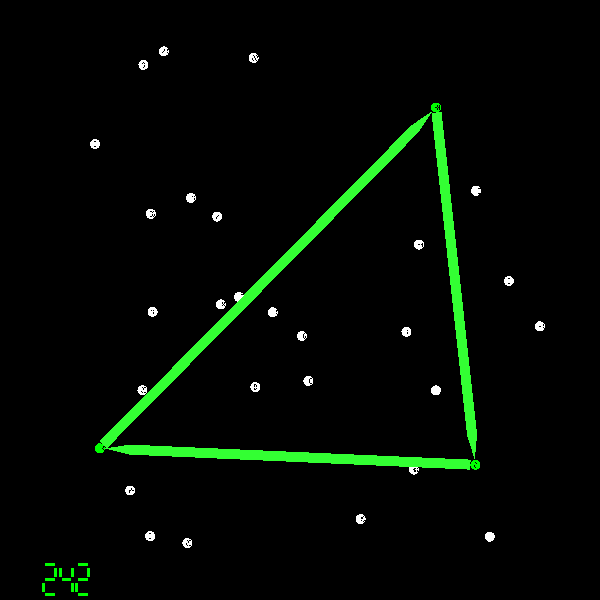
\includegraphics[width=29mm]{images/progress-00.png} &
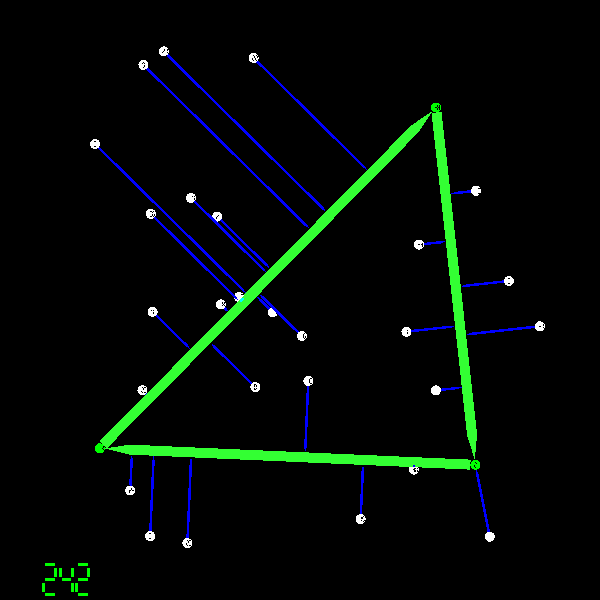
\includegraphics[width=29mm]{images/progress-01.png} &
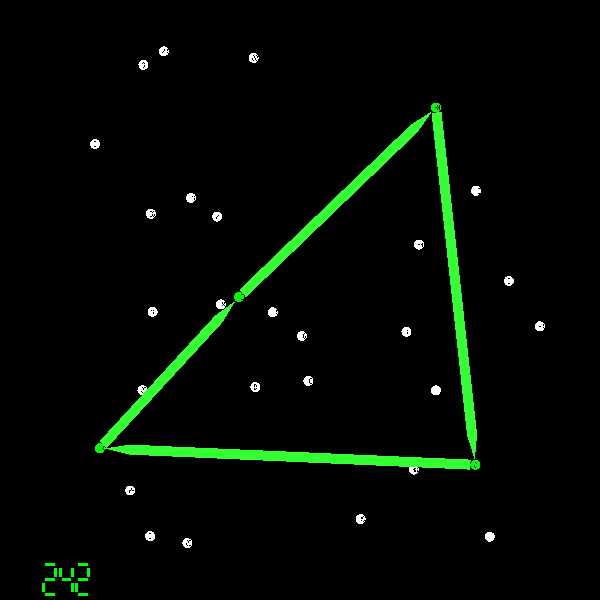
\includegraphics[width=29mm]{images/progress-02.png} &
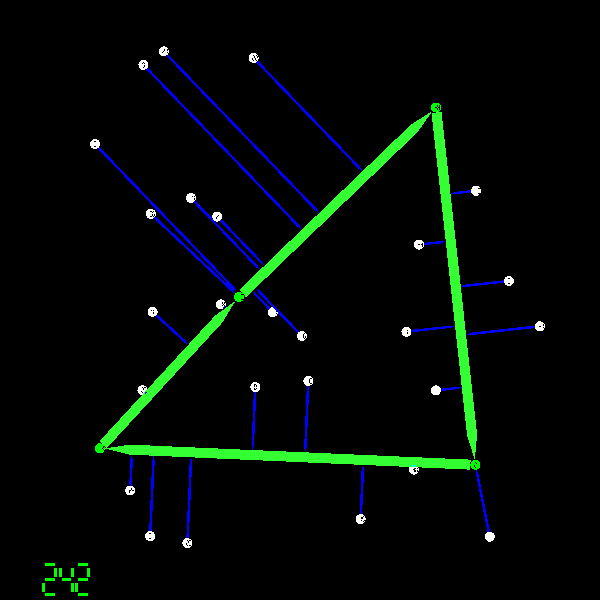
\includegraphics[width=29mm]{images/progress-03.png} \\
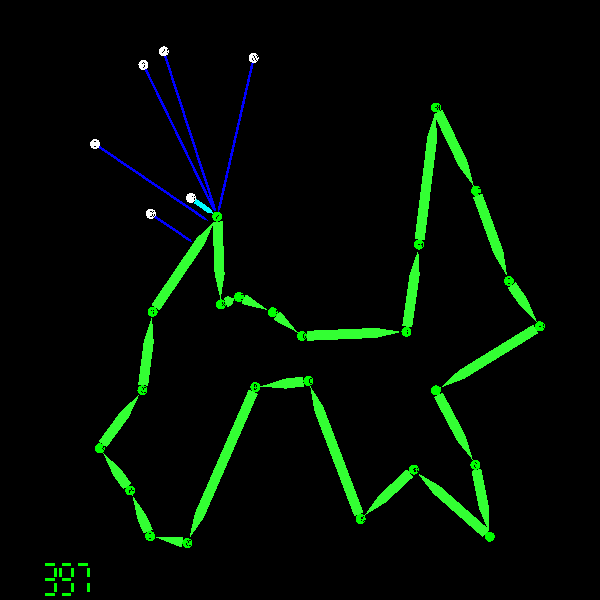
\includegraphics[width=29mm]{images/progress-04.png} &
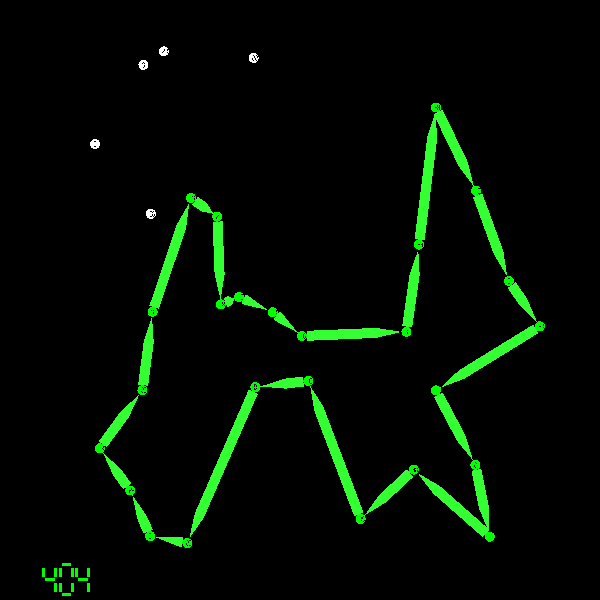
\includegraphics[width=29mm]{images/progress-05.png} &
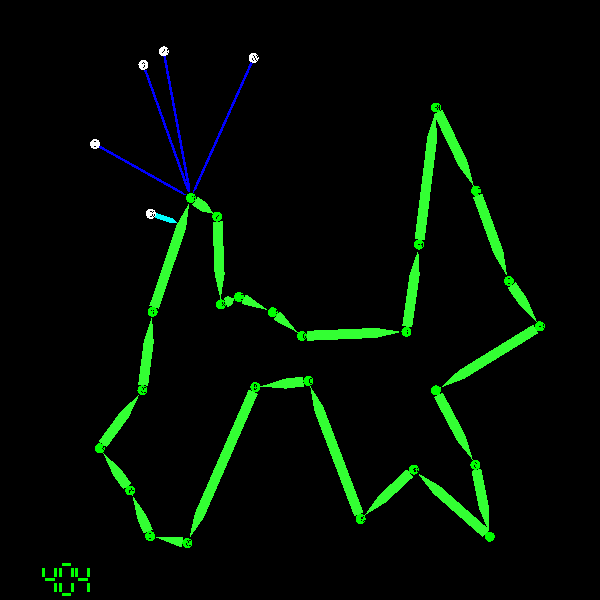
\includegraphics[width=29mm]{images/progress-06.png} &
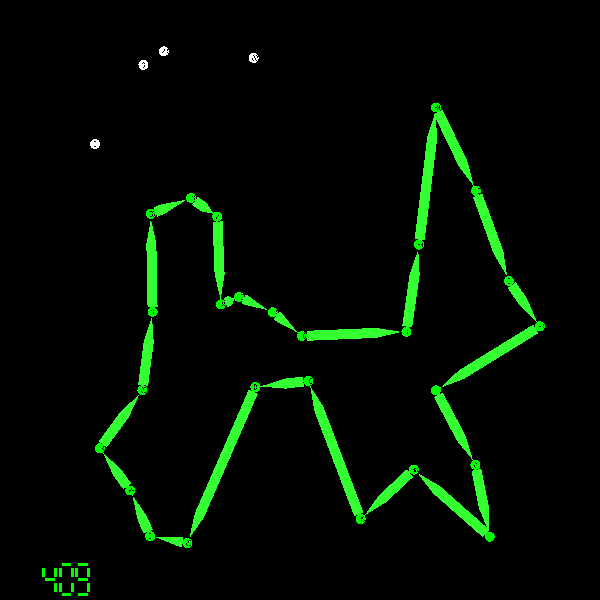
\includegraphics[width=29mm]{images/progress-07.png} \\
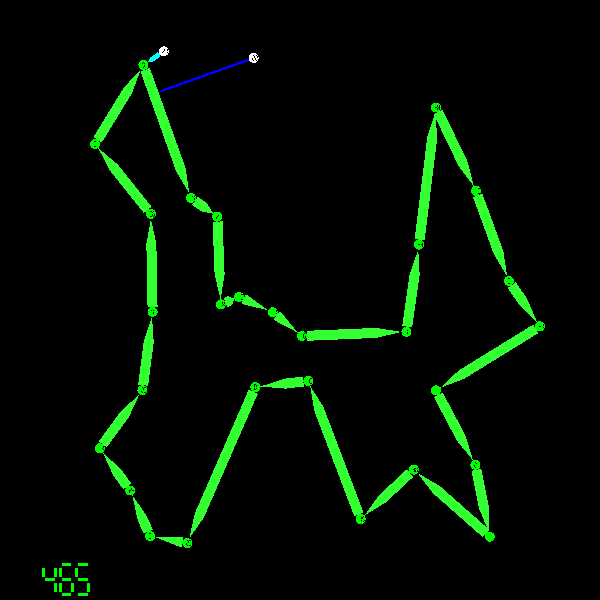
\includegraphics[width=29mm]{images/progress-08.png} &
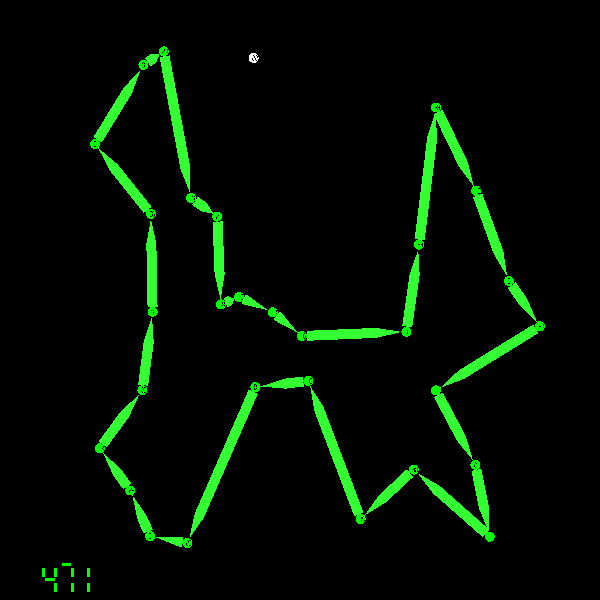
\includegraphics[width=29mm]{images/progress-09.png} &
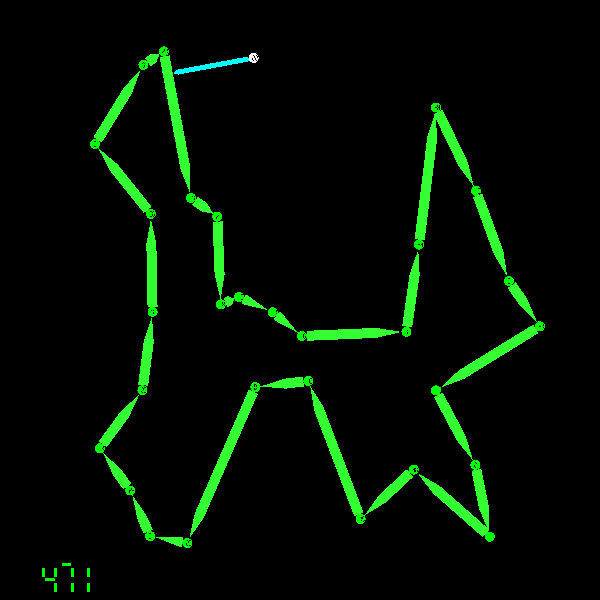
\includegraphics[width=29mm]{images/progress-10.png} &
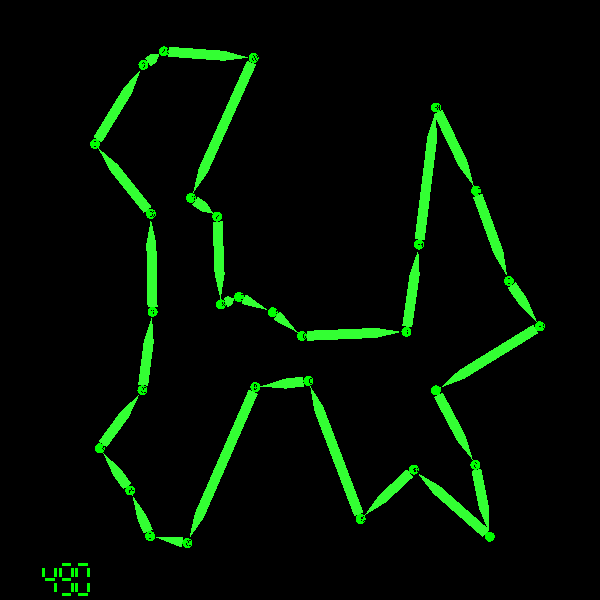
\includegraphics[width=29mm]{images/progress-11.png} \\
\end{tabular}
\caption{Progressive building of a solution, reads left to right, top to bottom. Starting at the top left, the initial
randomly selected 3 points form the starting triangle. In 3-nearest mode, the program instead picks one point and selects
the two points closest to it and uses that as the starting triangle. In the next pane, blue lines show the distance from
each point outside the path to the nearest edge. That point is added to the path and the repeats until all points
are added. Also notice the solution cost displayed in the bottom left corner of each pane.}
\label{fig:progress}
\end{center}
\end{figure}

%% template for 2 historgram plots
\newcommand{\myhist}[7]{%
    \begin{tikzpicture}
    \begin{axis}[
      at={(2.7cm, 0)},
      title=#1,
      ybar interval,
      height=8cm,width=14cm,
      enlargelimits=0.05,
      ybar interval=0.7,
      xtick=,% reset from ybar interval
      xmin=#2,xmax=#3,
      xticklabel=
    \pgfmathprintnumber\tick
    ]
    \addplot+[hist={bins=10,data=x}]
        file {#4};
    \addplot+[hist={bins=10,data=x}]
        file {#5};
    \legend{Nearest 3, Random 3}
    \end{axis}
    \node[label=#7, inner sep=0pt] (best) at (0,3)
        {\includegraphics[width=.25\textwidth]{#6}};
    \end{tikzpicture}
}

\begin{figure}
\myhist{30 Point Solution Cost Histogram}{480}{580}{plotdata/near-30.dat}{plotdata/rand-30.dat}
{images/rand-30.png}{Best 30 Point Solution}
\myhist{40 Point Solution Cost Histogram}{580}{680}{plotdata/near-40.dat}{plotdata/rand-40.dat}
{images/rand-40.png}{Best 40 Point Solution}
\caption{Cost of all candidate solutions for 30 and 40 point TSP. Blue column are cost for runs starting with 3 points
nearest to each other, red is for 3 points selected at random. The spread is about 10 units from best to worst in both
problems, indicating that this algorithm is fairly sensitive to initial conditions.}
\label{fig:hist}
\end{figure}

\section{Discussion}

Greedy algorithms run in sub-exponential time, and give acceptable solutions to NP-complete problems. Designing good and
fast selection heuristics is also important - even $N^3$ can get expensive for large problems and a linear or log-linear
solution become desirable for extremely large problems. In this project we showed the problems of size 30 and 40 can be
quickly solved by greedy selection based on distance to an edge, and that initial conditions for such an algorithm are
an important consideration.

\bibliographystyle{unsrt}  
\bibliography{references}

\end{document}
